\documentclass[tikz]{standalone}
\begin{document}
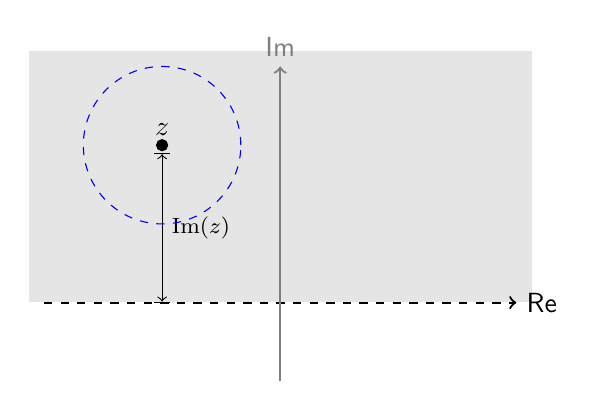
\begin{tikzpicture}
 
    \draw[color=white,fill=gray!20] (-3.2,0) -- (3.2,0) -- (3.2,3.2) -- (-3.2,3.2) -- (-3.2,0);
   \draw[->,thick,dashed] (-3,0) --  (3,0) node[right]{$\mathsf{Re}$} ;
     \draw[->,thick,gray] (0,-1) -- (0,3) node[above]{$\mathsf{Im}$};
\draw[fill] (-1.5,2) circle(2pt) node[above]{$z$};
\draw[|<->|] (-1.5,1.9) -- node[midway, right,font=\footnotesize]{$\mathrm{Im} (z)$} (-1.5,0);
\draw[dashed,color=blue] (-1.5,2) circle (1);
\end{tikzpicture}
\end{document}